%Do not change these lines, just uncomment the needed one
%\documentclass[prd,twocolumn,showpacs,groupedaddress,superscriptaddress,amsmath,amssymb]{revtex4-2}
\documentclass[prd,showpacs,groupedaddress,superscriptaddress,amsmath,amssymb]{revtex4-2} % one-column text
%\documentclass[preprint,showpacs,amsmath,amssymb]{revtex4-2}

\usepackage{hhline}
\usepackage{slashed}
\usepackage{graphicx}% Include figure files
\usepackage{graphics}
\usepackage{dcolumn}% Align table columns on decimal point
\usepackage{bm}% bold math
\usepackage{amssymb}
\usepackage{enumerate}
\usepackage{lineno}
\usepackage{multirow}
%\usepackage{footnote}

%\linenumbers


\textwidth19.0cm
\textheight24.0cm
\setlength{\topmargin}{-1.5cm}
\oddsidemargin -1.cm
\evensidemargin 2.cm
\def\u{\tilde{u}}
\def\s{\tilde{s}}
\def\t{\tilde{t}}
\def\P{\mathcal{P}}
\def\u{\tilde{u}}
\def\s{\tilde{s}}
\def\t{\tilde{t}}
\def\k{{\bf k}}
\def\p{{\bf p }}
\def\V{{\bf V}}

\newcommand\ee{e^+e^-}
\newcommand\xdecay{X \rightarrow e^+  e^-}
\newcommand\ainv{A'\to invisible}
\newcommand\inv{ \chi\overline{\chi}}
\newcommand\gp{ A'}
\newcommand\g{\gamma}
\newcommand\ma{m_{A'}}
\newcommand\pair{e^+e^-}
\newcommand\na{{n}_{A'}}
\newcommand\Na{{N}_{A'}}
\newcommand\ea{e^- Z \to e^- Z A';~ A' \to \chi \overline{\chi}}
\newcommand\emu{e^- Z \to e^- Z \g; \g \to \mu^+ \mu^-}
\newcommand\mm{\mu^+ \mu^-}


\begin{document}


%For CERN preprint:
%\begin{center}
%{\Large EUROPEAN ORGANIZATION FOR NUCLEAR RESEARCH}
%\end{center}
%\vskip1.5cm
%\begin{flushright}
%CERN-EP-2019-.....\\
%\today
%\end{flushright}
%end CERN preprint


\title{ \bf Study of sensitivities of the P2O project}


\author{M.~M.~Kirsanov$^{1}$\thanks{{\bf e-mail}: mikhail.m.kirsanov@gmail.com}, A.~Sokolov$^{2}$
\\
 $^1$ Institute for Nuclear Research of the Russian Academy of Sciences, \\117312 Moscow, Russia \\
 $^2$ Institute for High Energy Physics, Protvino, Russia \\
}


%alternative way of writing authors list, with a possibility of e-mail for several authors 
%\author{M. M. Kirsanov}
%\thanks{Corresponding author}
%\email[\textbf{e-mail}: ]{mikhail.kirsanov@cern.ch}
%\affiliation{Institute for Nuclear Research, 117312 Moscow, Russia}
%\author{N.~V.~Krasnikov}
%\email[\textbf{e-mail}: ]{nikolai.krasnikov@cern.ch}
%\affiliation{Institute for Nuclear Research, 117312 Moscow, Russia}
%\affiliation{Joint Institute for Nuclear Research, 141980 Dubna, Russia}


%For the collaboration papers:
%\input ../AUTHORS/author_list.tex


\date{\today}% It is always \today, today,
             %  but any date may be explicitly specified
%\date{June 17, 2009}% It is always \today, today,
             %  but any date may be explicitly specified



\begin{abstract}
The sensitivities of the project to some oscillation parameters as a function of power and systematic errors are studied.
\end{abstract}


\maketitle
\newpage


\section{Introduction}


 P2O is the project \cite{Akindinov:2019flp} of neutrino beam from IHEP Protvino to KM3NeT/ORCA \cite{KM3NET}


\section{Technical notes on the repository}


 The files for this project, including Papers and Notes, are kept in https://github.com/kirsanov-protvino/P2O . In order to work
on them one should create account on github. Next step is to create an SSH key. Add this key to your account on the page https://github.com/settings/keys.
After that you will be able to clone the repository using the command git clone git@github.com:kirsanov-protvino/P2O.git and push your changes in it.
The command above is shown when you click the green button "Code" on the repository page and switch to SSH instead of HTTPS.
To check that your repositiry clone is "pushable" type inside it "git remote -v".


\section{Technical notes on the Globes program running}


 In order to check that the statistics corresponds to the Proposal, the following call was used: \\
glbGetChannelRatePtr(0, ichannel, GLB\_PRE).
It returns the numbers of events in energy bins, to be summed over the them. It is to be called AFTER the calculation of sensitivities,
otherwise some variables are not initialized. It is found that with the normalization factor 40 in the glb file the total number of
events corresponds to the one in Figure 7 of the Proposal \cite{Akindinov:2019flp} (20000 $\nu_{\mu}CC$ events by eye from the figure,
after scaling from 90 MW to 450 MW).

 In the Globes running the file p2o.glb was used. Some parameters there, such as energy resolution of 30\%, are taken from the
Proposal \cite{Akindinov:2019flp}, some from the proposal of KM3NET https://iopscience.iop.org/article/10.1088/0954-3899/43/8/084001.


\section{Study of the experiment resolution}


 The parameters of the proposed experiment are described in \cite{Akindinov:2019flp} and \cite{KM3NET}. Some of them can be changed,
for example the detector mass (several construction stages are possible), others, such as the energy resolution, and identification probabilities,
are more difficult to change. However, there are ideas how to improve them, and may be significantly \cite{Perrin_Terrin_2022}.
For this reason we studied how the results, in particular the $\delta$ CP measurement, depend on the experiment parameters.
 The value of $\sqrt{\chi^2}$ as a function of hypothetical $\delta$ for the true values $\delta = \pi/2, \pi, 3\pi/2$ is shown
in Fig. \ref{fig:del}. The energy resolution here is nominal, 30\%, as specified in the Proposal. Here, only neutrino exposition is used.

\begin{figure*}[h]
\begin{center}
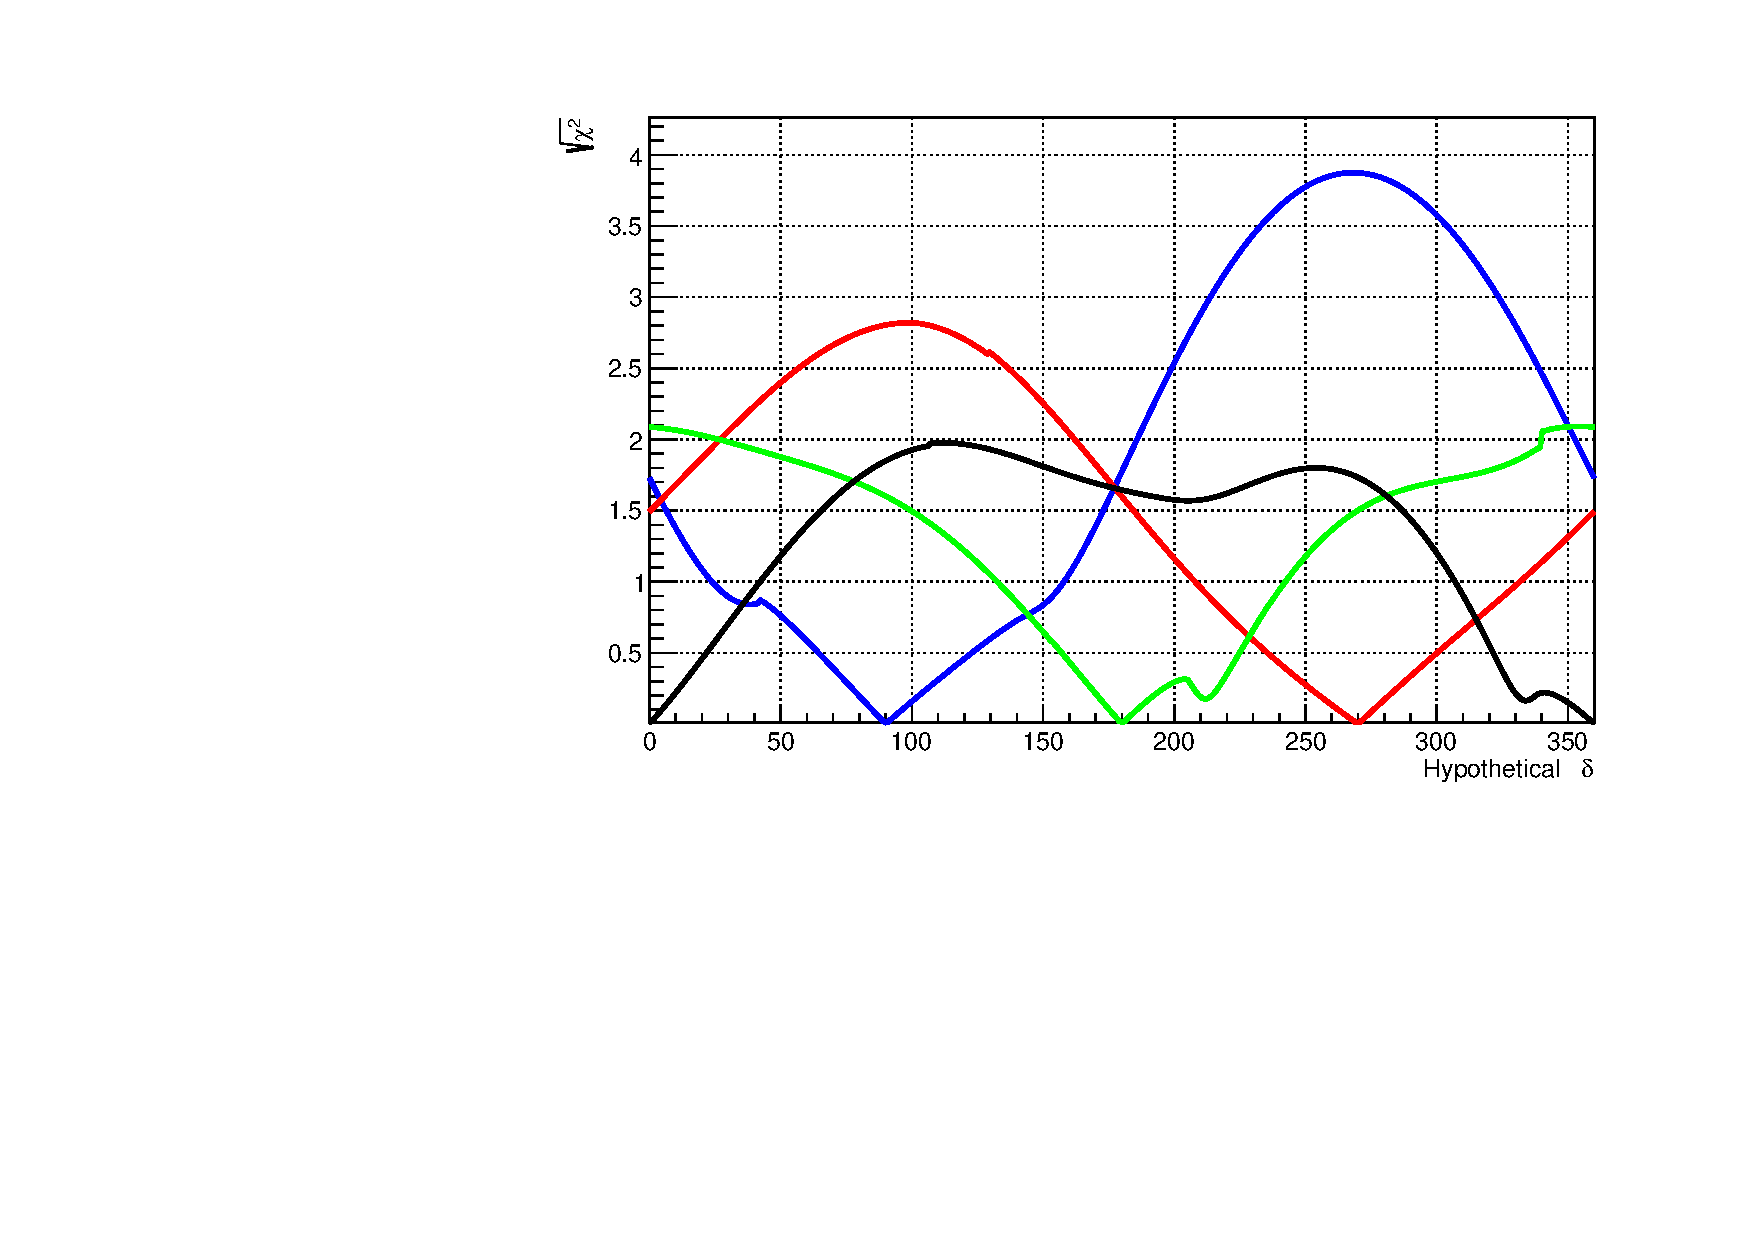
\includegraphics[width=0.75\textwidth]{del.pdf}
\caption {Value of $\sqrt{\chi^2}$ as a function of hypothetical $\delta$ for $\delta = \pi/2$ (blue), $\pi$ (green), $3\pi/2$ (red). Energy resolution is 30\%.
\label{fig:del}}
\end{center} 
\end{figure*}

 For comparison, we tried to add the antineutrino exposition (1/3 of the neutrino one). The result is in Fig. \ref{fig:del_anu}. Here, in addition,
the energy cut at 2 GeV was used here. In order to keep the same number of $\nu_{\mu}CC$ events the Globes neutrino flux normalization is increased from 40 to 50.
We checked that equal exposition of neutrino and antineutrino does not change the result. Here, also the correct distribution of the NC visible energy
(for simplicity y distribution is assumed uniform from 0 to 1) is implemented.

\begin{figure*}[h]
\begin{center}
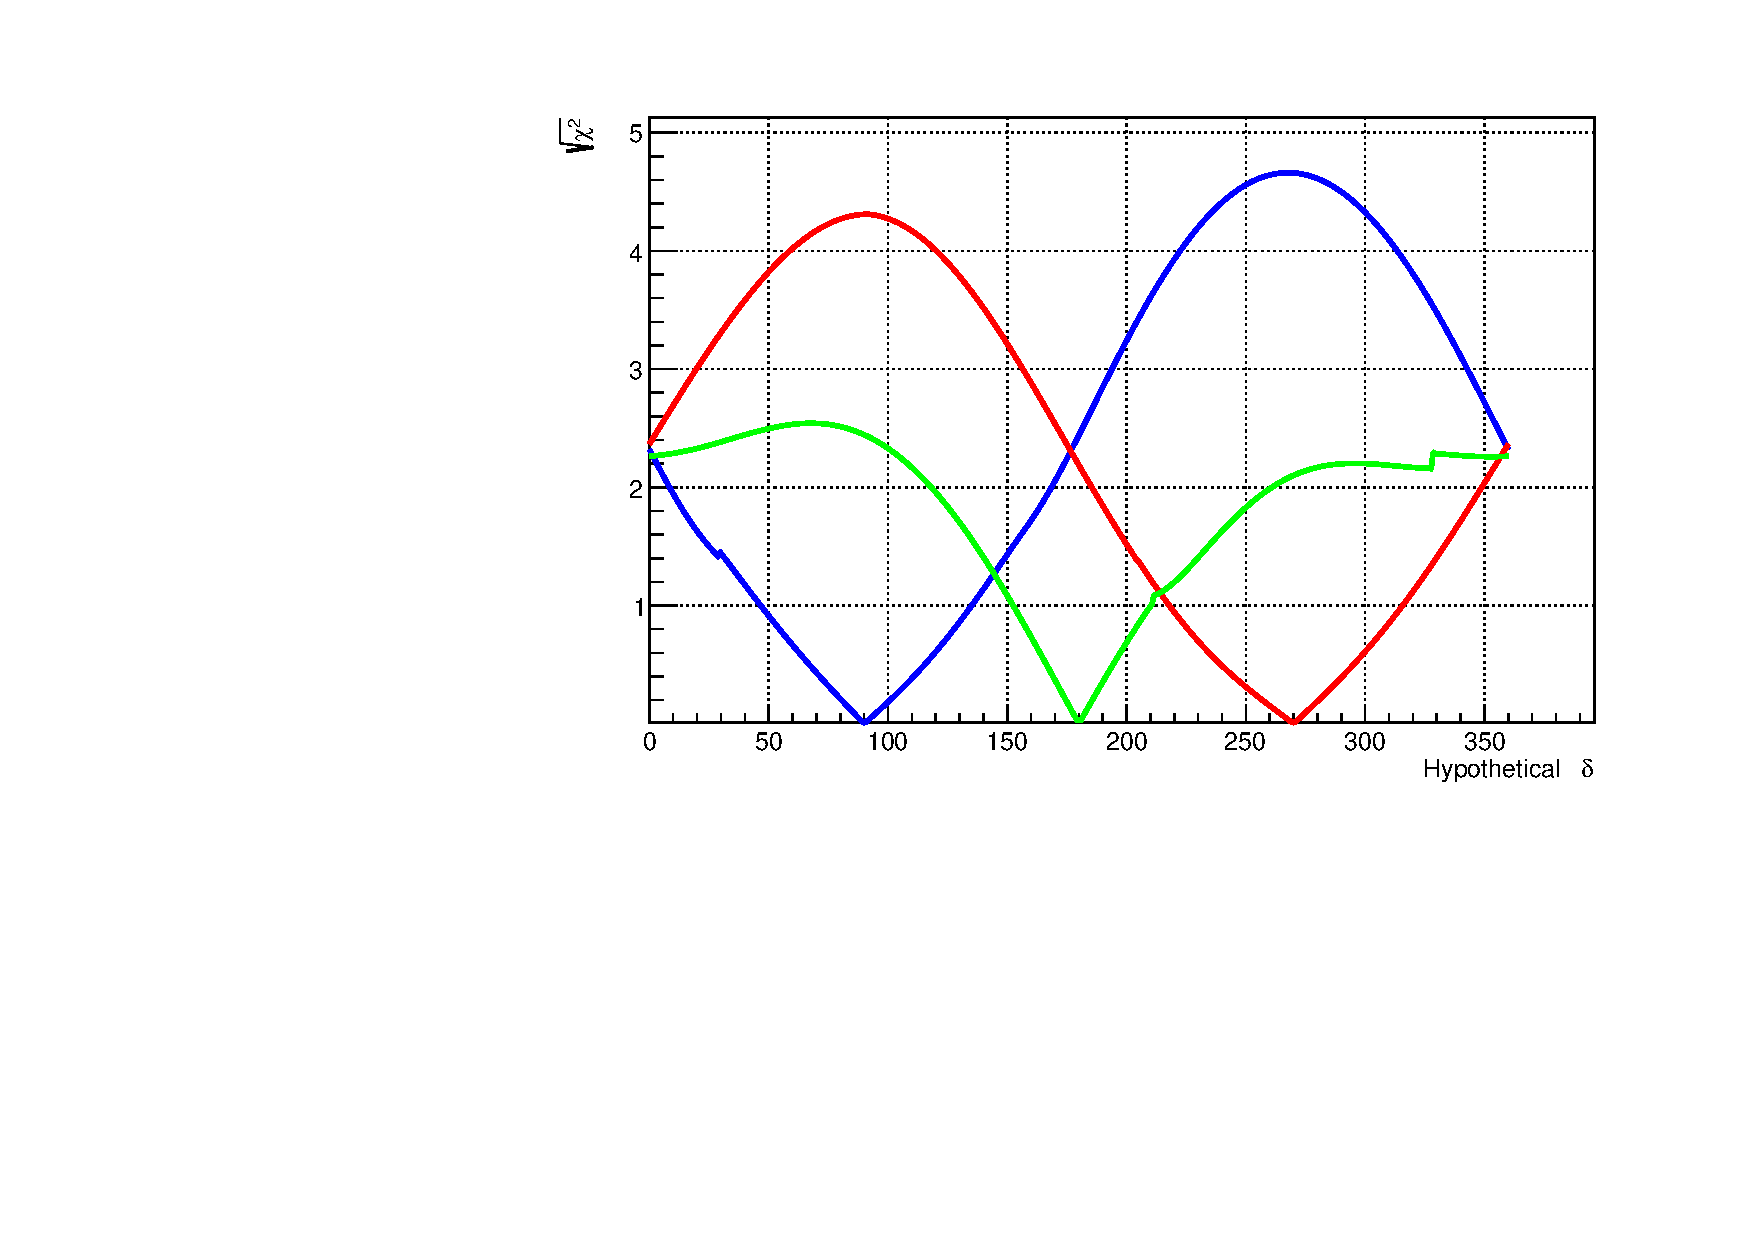
\includegraphics[width=0.75\textwidth]{del_anu.pdf}
\caption {Value of $\sqrt{\chi^2}$ as a function of hypothetical $\delta$ for $\delta = \pi/2$ (blue), $\pi$ (green), $3\pi/2$ (red).
          The antineutrino exposition 1/3 of neutrino one is added. In addition, the energy cut at 2 GeV is applied in the analysis. Energy resolution is 30\%.
          The corresponding resolutions on $\delta$ measurements are: 44.55, 28.8, 48.6 degrees.
\label{fig:del_anu}}
\end{center}
\end{figure*}

 One of the main purposes of the experiment is the measurement of $\delta$ CP. It is determined as the deviation of $\delta$ from the minimum
of $\chi^2$ at which the latter increases by 1, averaged over the left and right sides.

 We studied the dependence of $\delta$ resolution on the fraction of antineutrino exposition in the total exposition. The result
is shown in Fig. \ref{fig:del_delres_anufrac}.

\begin{figure*}[h]
\begin{center}
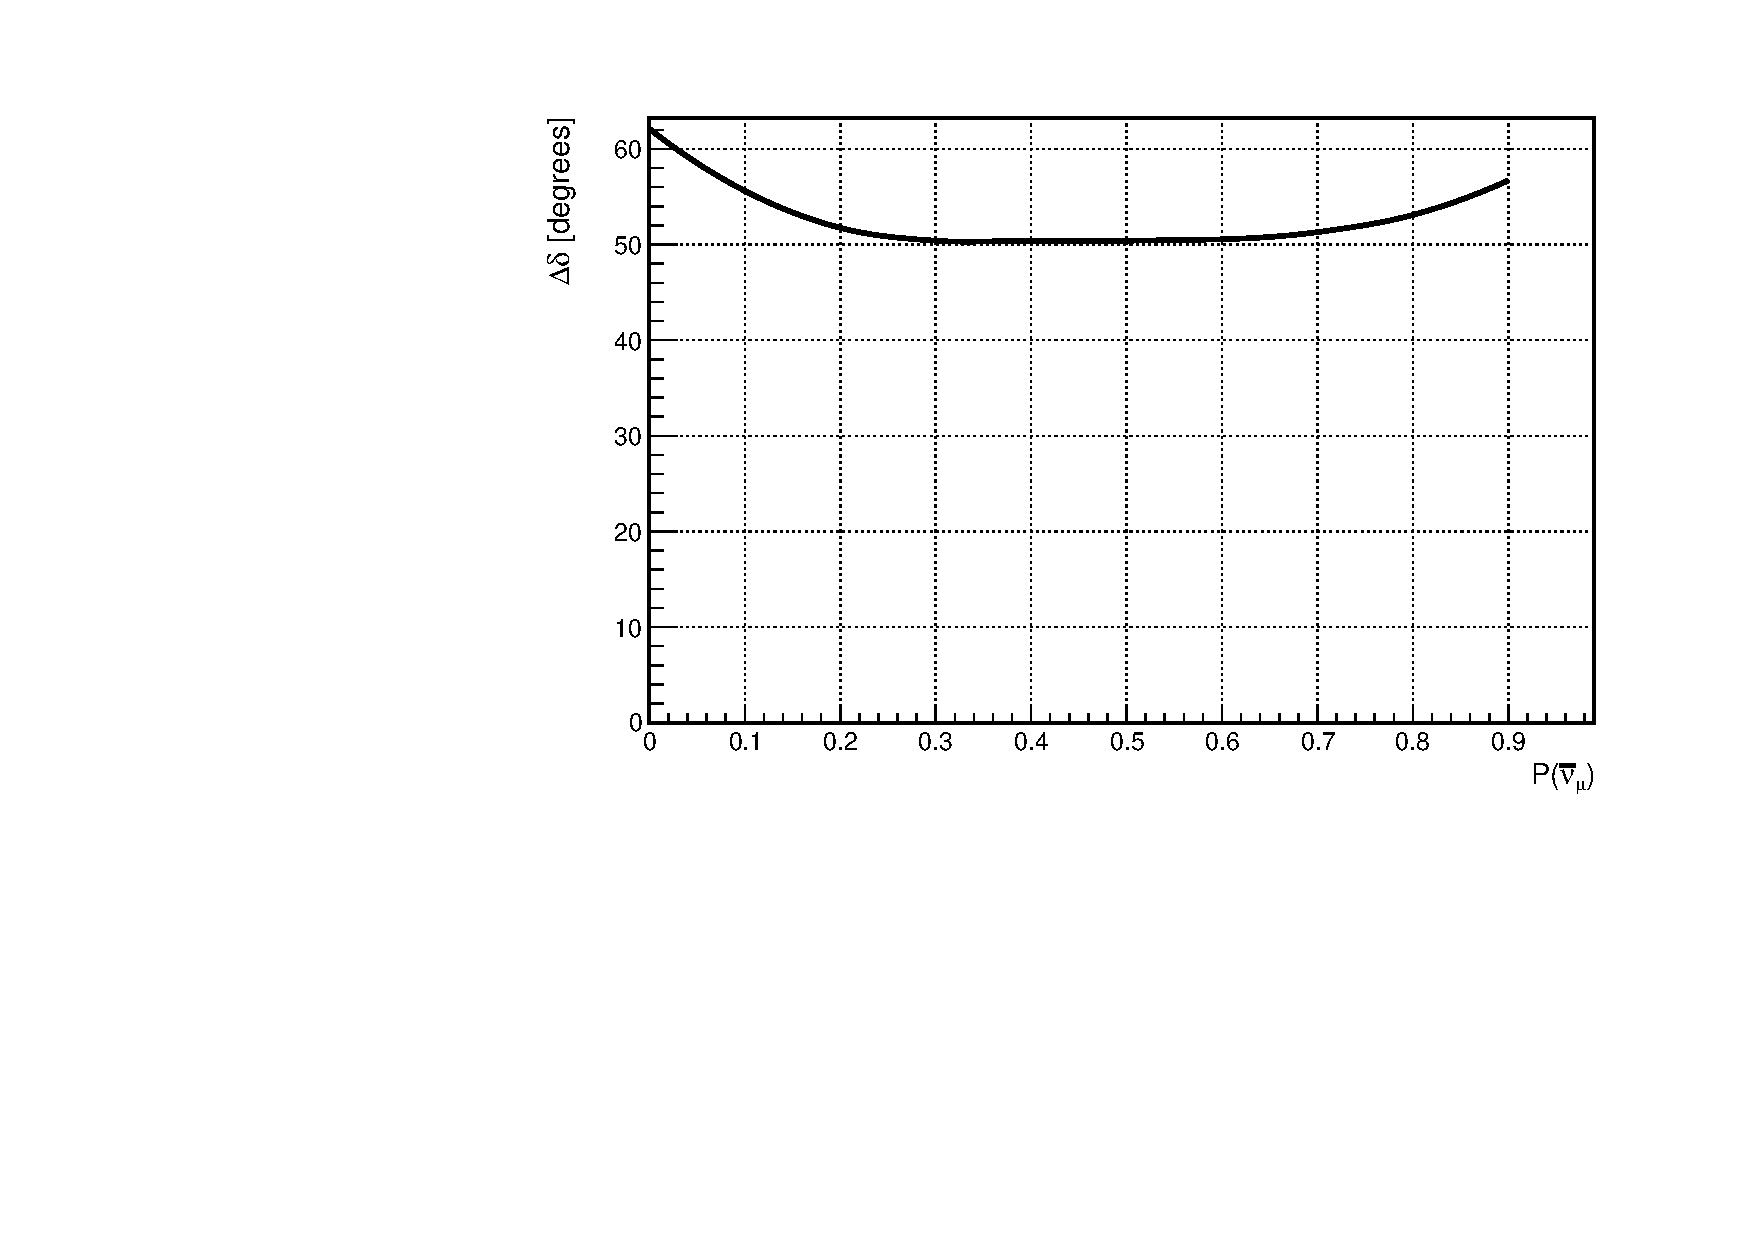
\includegraphics[width=0.75\textwidth]{del_delres_anufrac.pdf}
\caption {Resolution of the $\delta$ CP measurement as a function of the antineutrino exposition fraction for the true value $\delta = 3\pi/2$.
\label{fig:del_delres_anufrac}}
\end{center}
\end{figure*}

 The resolution of $\delta$ measurement for the true values $\delta = 0, \pi/2, \pi, 3\pi/2$ is shown in Fig. \ref{fig:del_delres_eres}.

\begin{figure*}[h]
\begin{center}
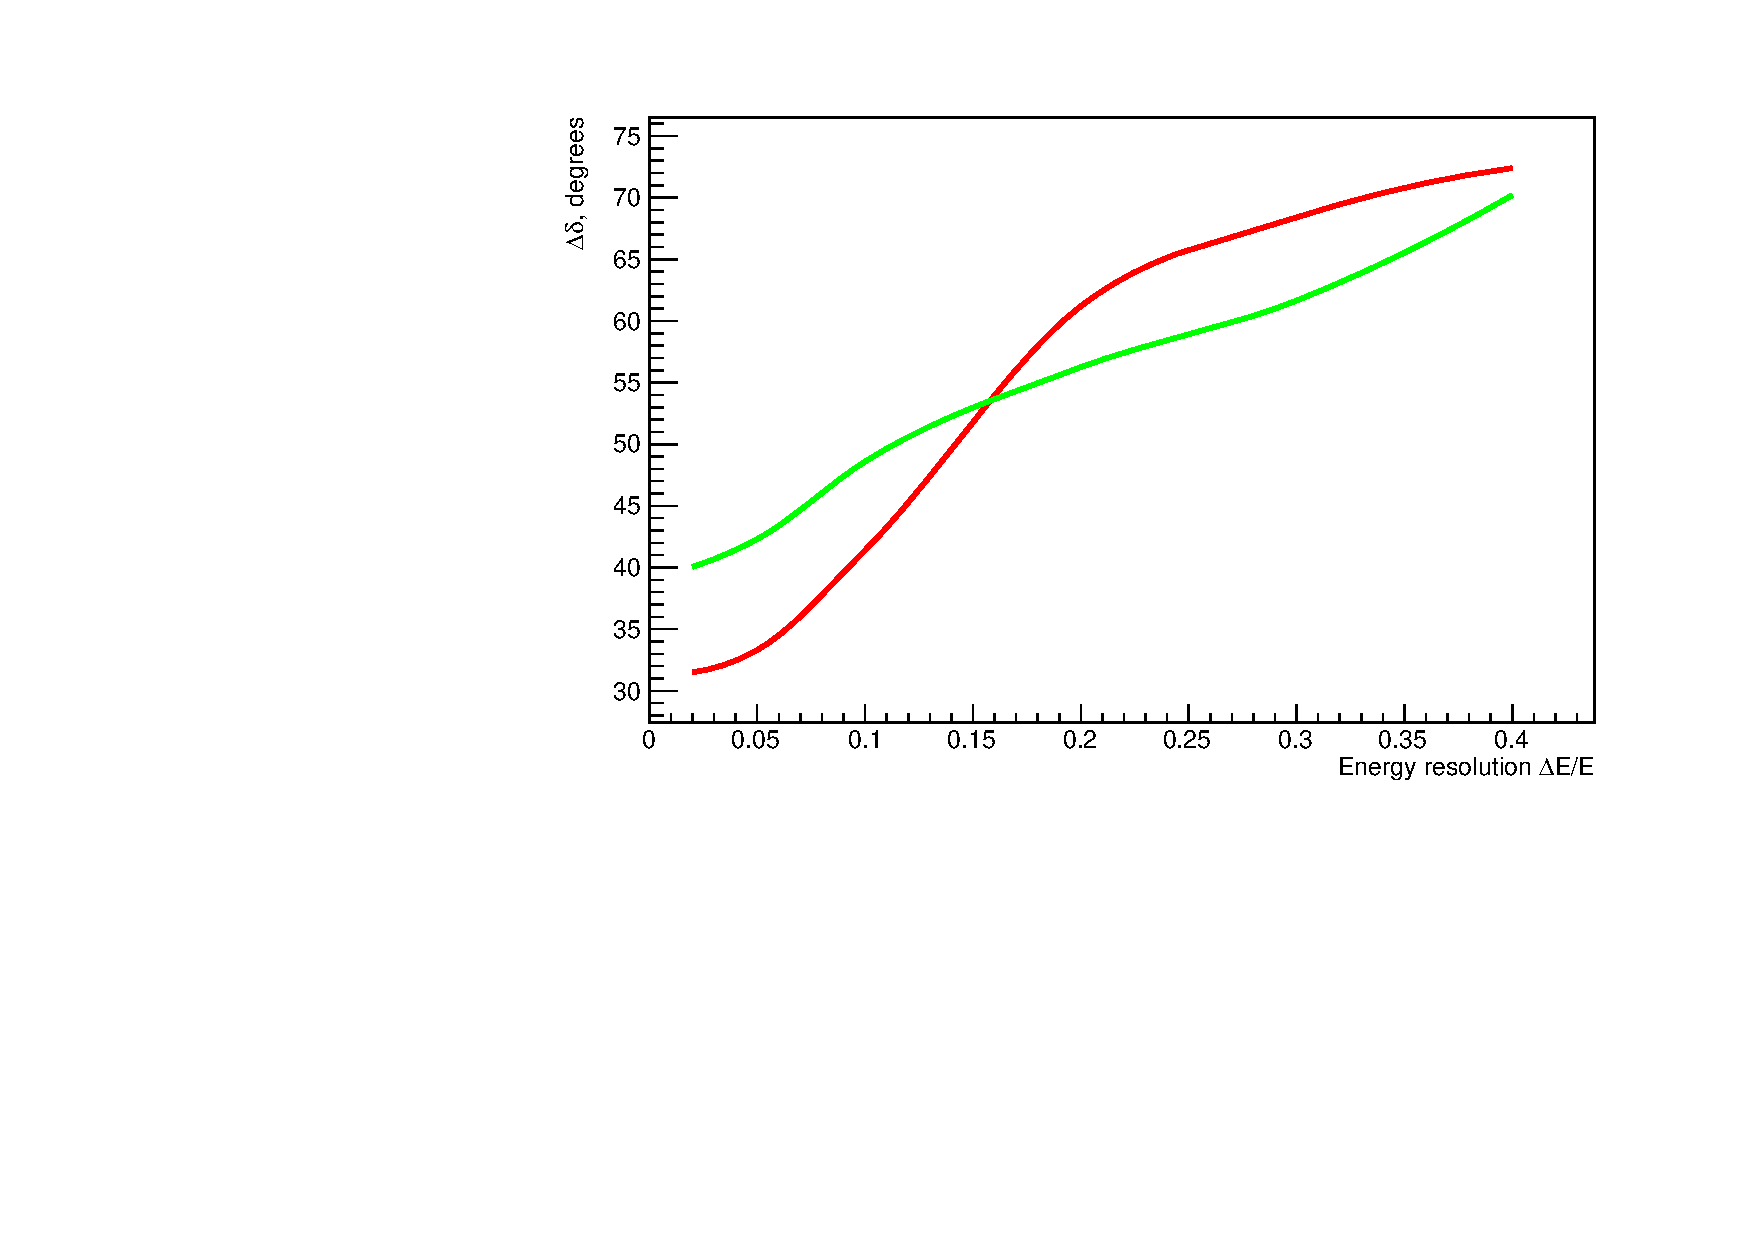
\includegraphics[width=0.75\textwidth]{del_delres_eres.pdf}
\caption {Resolution of the $\delta$ CP measurement as a function of energy resolution for the true values $\delta = 0$ (black), $\pi/2$ (blue),
$\pi$ (green), $3\pi/2$ (red).
\label{fig:del_delres_eres}}
\end{center}
\end{figure*}

 The resolution of $\delta$ measurement as a function of the detector mass is shown in Fig. \ref{fig:del_delres_mdet}. The project detector mass is 8 mt.

\begin{figure*}[h]
\begin{center}
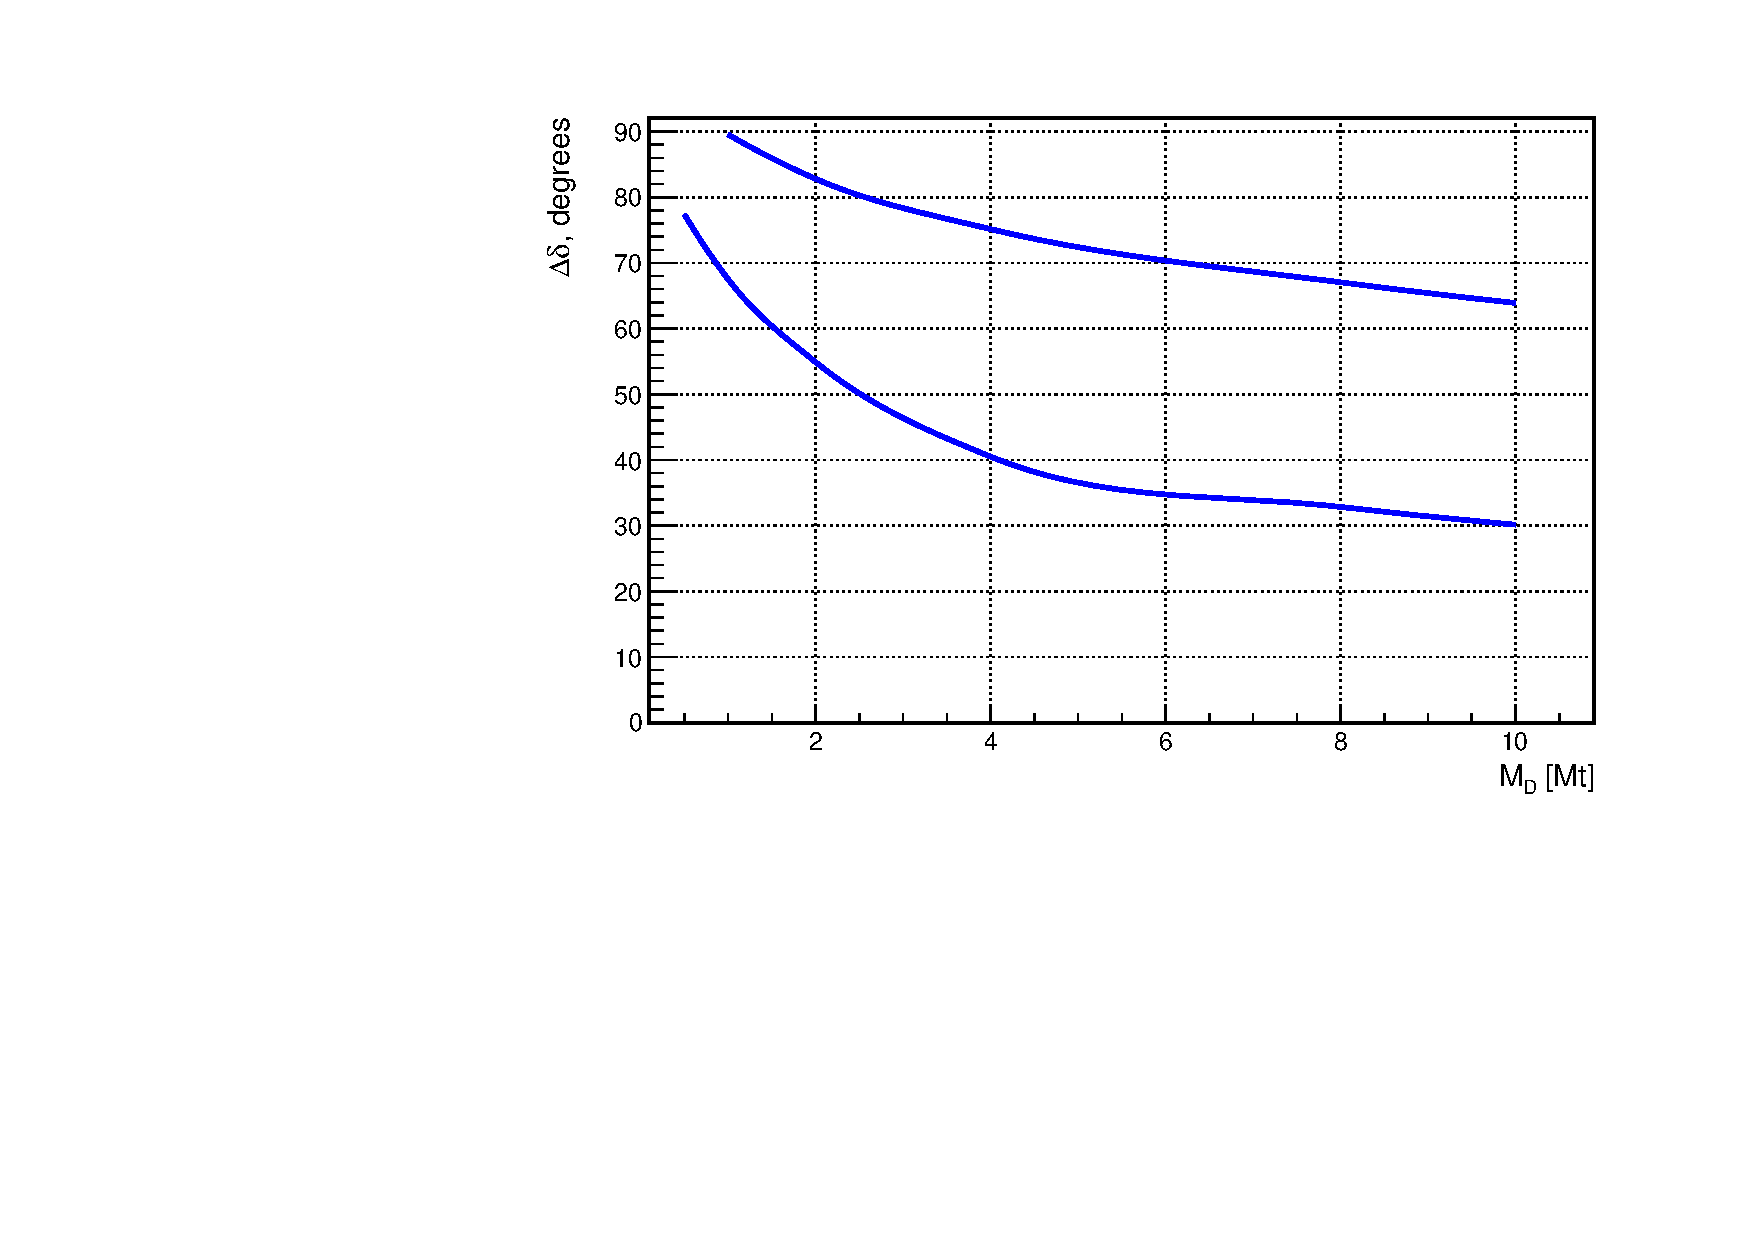
\includegraphics[width=0.75\textwidth]{del_delres_mdet.pdf}
\caption {Resolution of the $\delta$ CP measurement as a function of the detector mass for the true value $\delta = \pi/2$
and energy resolutions 0.3 (nominal value, upper curve) and 0.05 (lower curve).
\label{fig:del_delres_mdet}}
\end{center}  
\end{figure*}


\section{Effect of $\nu_e$ fraction in the beam}


This fraction is specified in the spectra file. To avoid rewriting the spectra files, different fractions were simulated by changing the efficiency
with which the channel "nu-e-beam" is added to the backgrounds. This is possible because the program does not have a protection against efficiencies
greater than 1. For example the nominal efficiency for the $\nu_e$ appearence is 0.85. The fraction of $\nu_e$ increased by factor of 10 was
simulated by increasing this efficiency to 8.5. This changes the delta CP measurement accuracy from 61.65 to 62.55 degrees (delta CP = 3/2 $\pi$).
Decreasing the $\nu_e$ fraction is not visible if we print out only 3 digits of delta CP measurement.

I understand this small effect like this. All events without identified muon are summed up ("shower type" events) and used in the analysis. In the model
described in our glb file we have one error specified for this: 5\%. So the effect of increased $\nu_e$ fraction remains small if the fraction of $\nu_e$
in the total number of "shower type" events does not dominate.

The effect of $\nu_e$ fraction can be more significant if we assume that we don't know it with sufficient accuracy and specify this separate accuracy
in the glb file. "Sufficient" here means a value of the order of 5\% mentioned above.


\section{Effect of the type of systematic error}


No significant effect was observed when it was changed from "chiSpectrumCalib" to "chiSpectrumTilt". Artefacts in the dependencies also did not change.



\clearpage
\bibliographystyle{apsrev4-2}
\bibliography{../Bibliography/bibliographyP2O}


\end{document}
